\documentclass[acmtog]{acmart}
\usepackage{graphicx}
\usepackage{subfigure}
% Title portion
\title{Assignment 4 - Global illumination using path tracing} 
\author{Name:\quad Su'an Xia  \\ student number:\quad 18047482
	\\email:\quad xiasa@shanghaitech.edu.cn}

% Document starts
\begin{document}
\maketitle

\vspace*{2 ex}


\section{Introduction}
\subsection{Ideal diffuse BRDF and ideal specular BRDF}
Requirement: Finish "evaluate" and "sample".
\\Main process: 
\\(1) Ideal diffuse BRDF's "evaluate()" and "sample()".
\\(2) Ideal specular BRDF's "evaluate()" and "sample()".

\vspace*{1 ex}
\subsection{Area light support}
Requirement: Implement an area light.
\\Main process:
\\(1) SampleSurfacePos();
\\(2) isHit();

\vspace*{1 ex}
\subsection{An integrator that utilizes path tracing to render image}
Requirement: Implement the following 2 functions.
\\Main process:
\\(1) rend();
\\(2) radiance();

\vspace*{2 ex}
\section{IMPLEMENTATION DETAILS}
\subsection{Ideal diffuse BRDF and ideal specular BRDF}
In material.hpp, we need to complete the 2 subclass 'IdealDiffuse' and   'IdealSpecular'.
\\In 'IdealDiffuse', for the 'sample()' function, we first generate 2 random variables, then calculate the  'r' and 'phi' based on the disk, next project it to the hemishpere. At last return the pdf. For the 'eval()' function, we just evaluate the BRDF by formula. It is easy.
\\Similarly, in 'IdealSpecular', we do the same thing but we only to sample in the opposite direction. The remaining thing is still the same.

\vspace*{1 ex}
\subsection{Area light support}
In light.hpp, we need to complete the subclass 'AreaLight'.
\\In 'SampleSurfacePos()' function, just like what we did in the section 1, we generate 2 random variables to sample a disk. Record the pdf and return the color. 
\\In 'isHit()' function, we need to determine if light is hit. We calculate the t and check whether it is within the scope.
\vspace*{1 ex}

\subsection{An integrator that utilizes path tracing to render image}
In pathTracingIntegrator.hpp, we need to complete the function 'render()' and 'radiance()'
\\In render(),for each pixel we should determine the final color. First we generate ray, then get the interaction. If is a glowing object, then break, else continue. Then we find next path vertex and accumulate contribution, intersect ray with scene and store intersection in isect, possibly add emitted light at intersection, add emitted light at path vertex or from the environment, terminate path if ray escaped or maxDepth was reached, sample illumination from lights to find path contribution,sample BSDF to get new path direction and finally possibly terminate the path with Russian roulette.
\\In radiance(), we mainly uniform sample one light. we randomly choose a single light to sample, then estimate Direct light. We sample light source with multiple importance sampling, compute BSDF or phase function’s value for light sample, add light’s contribution to reflected radiance, sample BSDF with multiple importance sampling, account for light contributions along sampled direction wi.

\vspace*{2 ex}

\section{Results}

\begin{figure}[h]
\centering
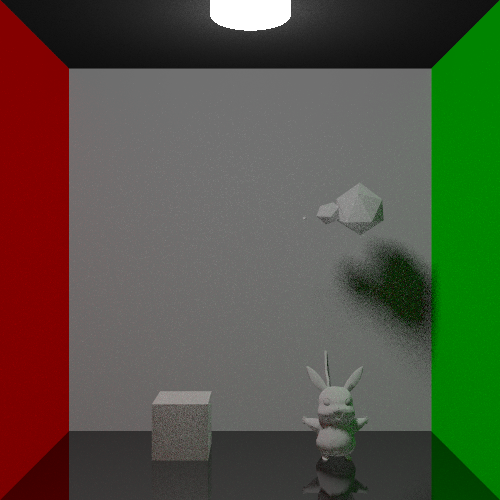
\includegraphics[width=6cm,height=8cm]{final.png}
\caption{Final}
\end{figure}


\end{document}
